%        File: pnas_appendix.tex
%     Created: Wed Oct 12 05:00 PM 2011 P
% Last Change: Wed Oct 12 05:00 PM 2011 P
%


%\documentclass[authoryear,5p]{elsarticle}
\documentclass[authoryear,review,11pt]{elsarticle}
\bibliographystyle{elsarticle-harv}
\usepackage{graphicx}
\usepackage{amsmath,amsfonts}
\usepackage{lineno}
\linenumbers
\usepackage{subfigure}
\usepackage[pdftex]{color}
\definecolor{darkblue}{rgb}{0,0,0.5}
\definecolor{darkgreen}{rgb}{0,0.5,0}
%\usepackage[pdftex, colorlinks, citecolor=darkblue,linkcolor=darkgreen]{hyperref}
\usepackage[pdftex, colorlinks]{hyperref}
\textwidth 6.75in
\oddsidemargin -0.15in
\evensidemargin -0.15in
\textheight 9in
\topmargin -0.5in
\newcommand{\ud}{\mathrm{d}}
\newcommand{\E}{\mathrm{E}}
\newcommand{\C}{\mathrm{Cov}}
\newcommand{\V}{\mathrm{Var}}


%\graphicspath{{/home/cboettig/Documents/ucdavis/research/phylotrees/images/}}

\journal{Proceedings of the National Academy of Sciences } 
\begin{document}
%\begin{frontmatter}
%  \title{  }
%  \author[cpb]{Carl Boettiger\corref{cor1}}
%  \author[alan]{Alan Hastings}
%  \ead{cboettig@ucdavis.edu}
%  \cortext[cor1]{Corresponding author.}
%  \address[cpb]{Center for Population Biology, University of California, Davis, United States}
%  \address[esp]{Department of Environmental Science and Policy, University of California, Davis, United States}
%\end{frontmatter}
%


\begin{figure}[ht]
  \begin{center}
    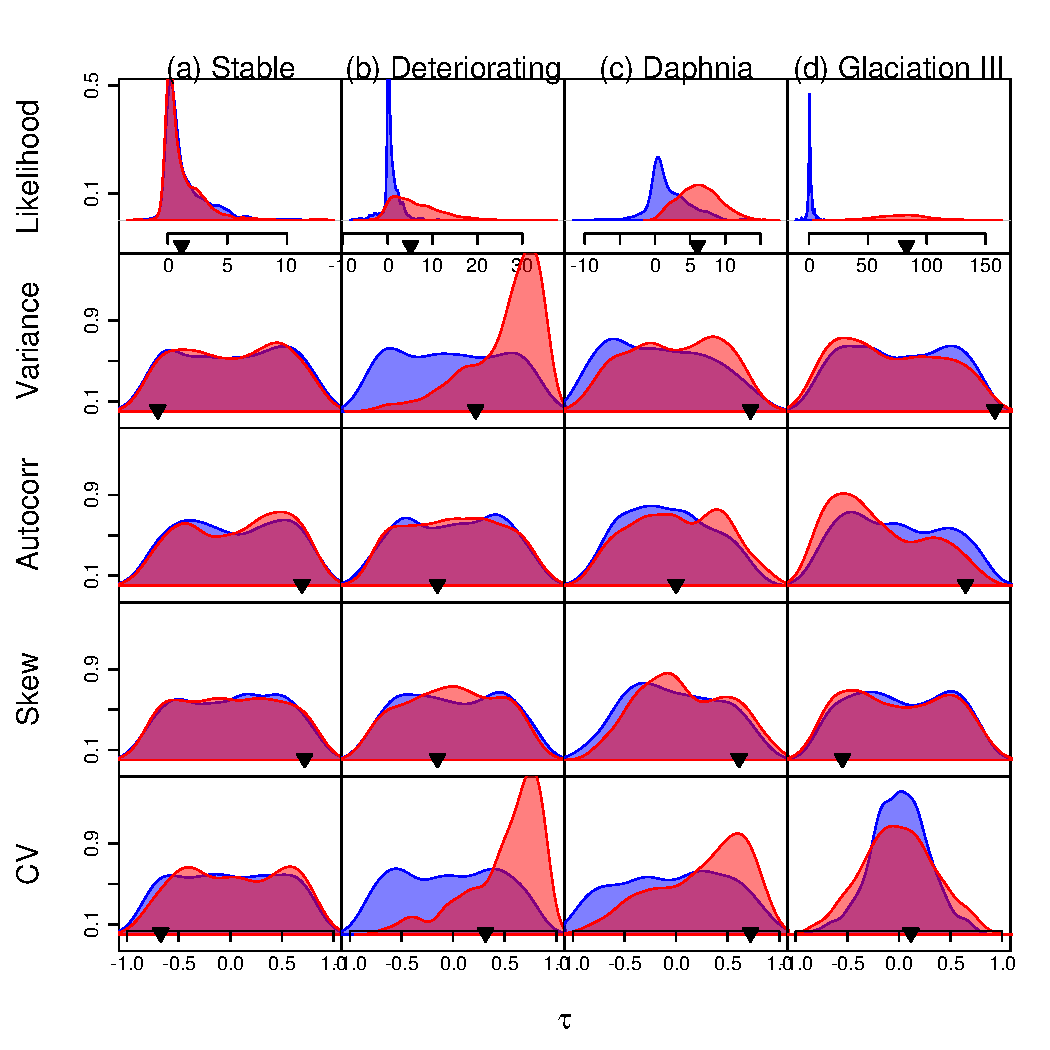
\includegraphics{FigS1.pdf}
  \end{center}
  \caption{Distribution of the indicator statistic}
  \label{fig:S1}
\end{figure}

\begin{figure}[ht]
  \begin{center}
    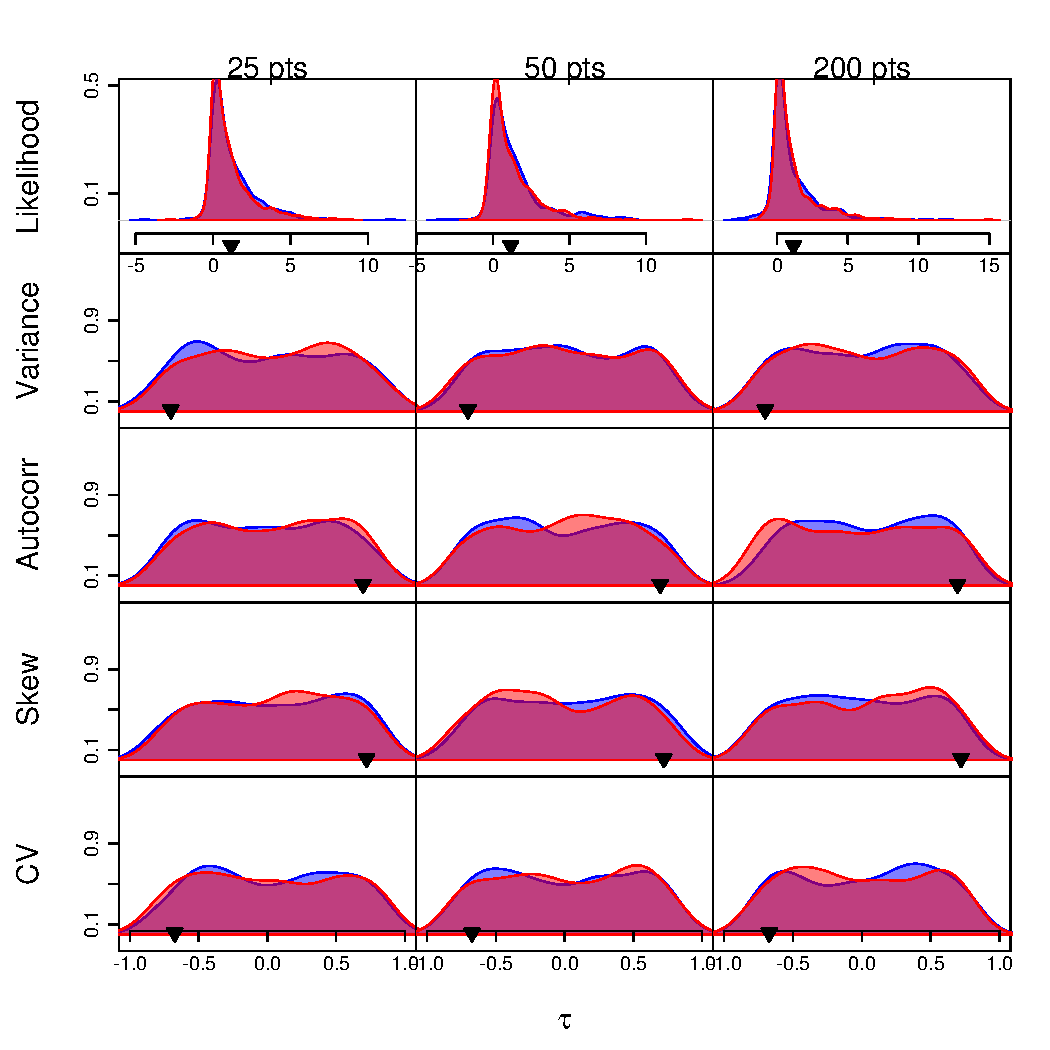
\includegraphics{FigS2.pdf}
  \end{center}
  \caption{Distributions of the indicator statistic as the sampling effort increases in the simulated data.}
  \label{fig:S2}
\end{figure}


\begin{figure}[ht]
  \begin{center}
    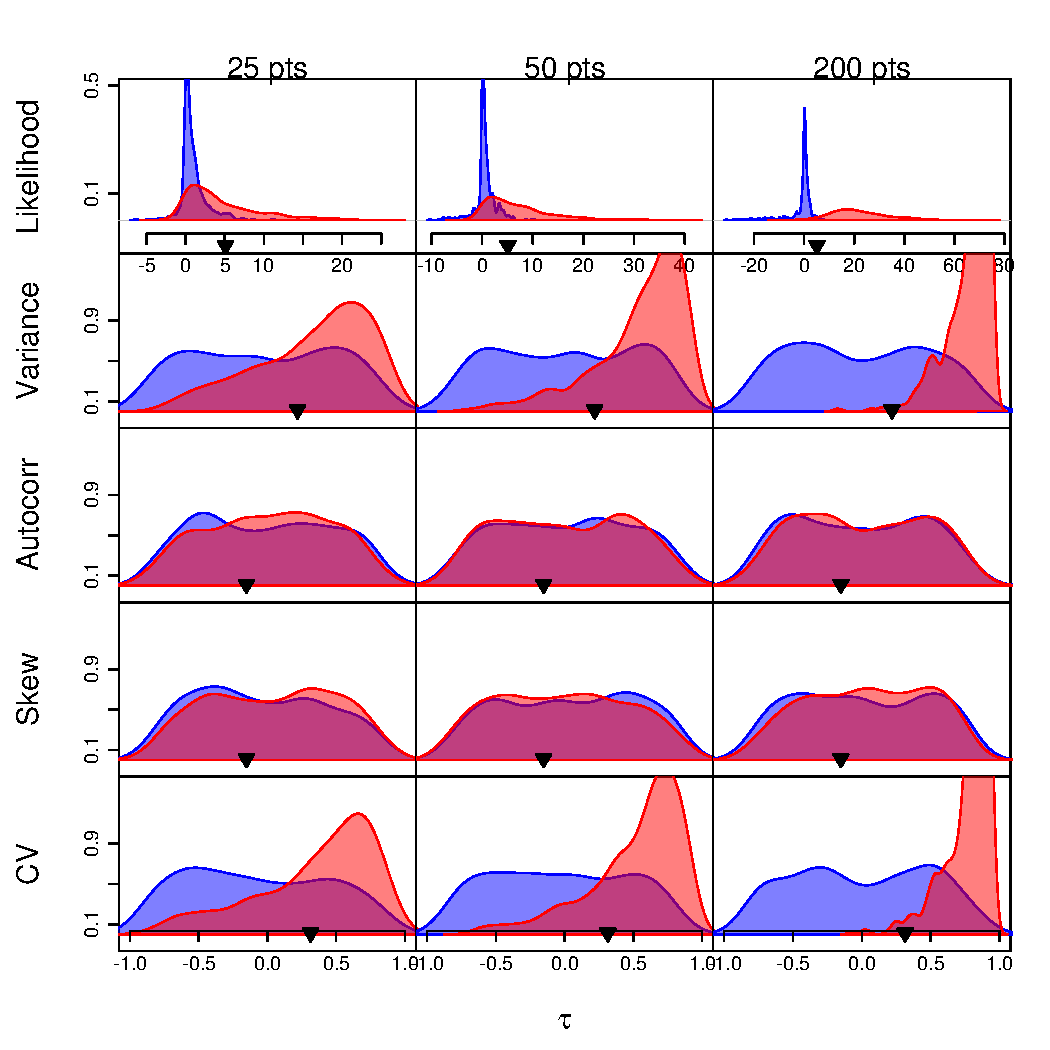
\includegraphics{FigS3.pdf}
  \end{center}
  \caption{Distributions of the indicator statistic as the sampling effort increases in the \emph{Daphnia} data.}
  \label{fig:S3}
\end{figure}


\begin{figure}[ht]
  \begin{center}
    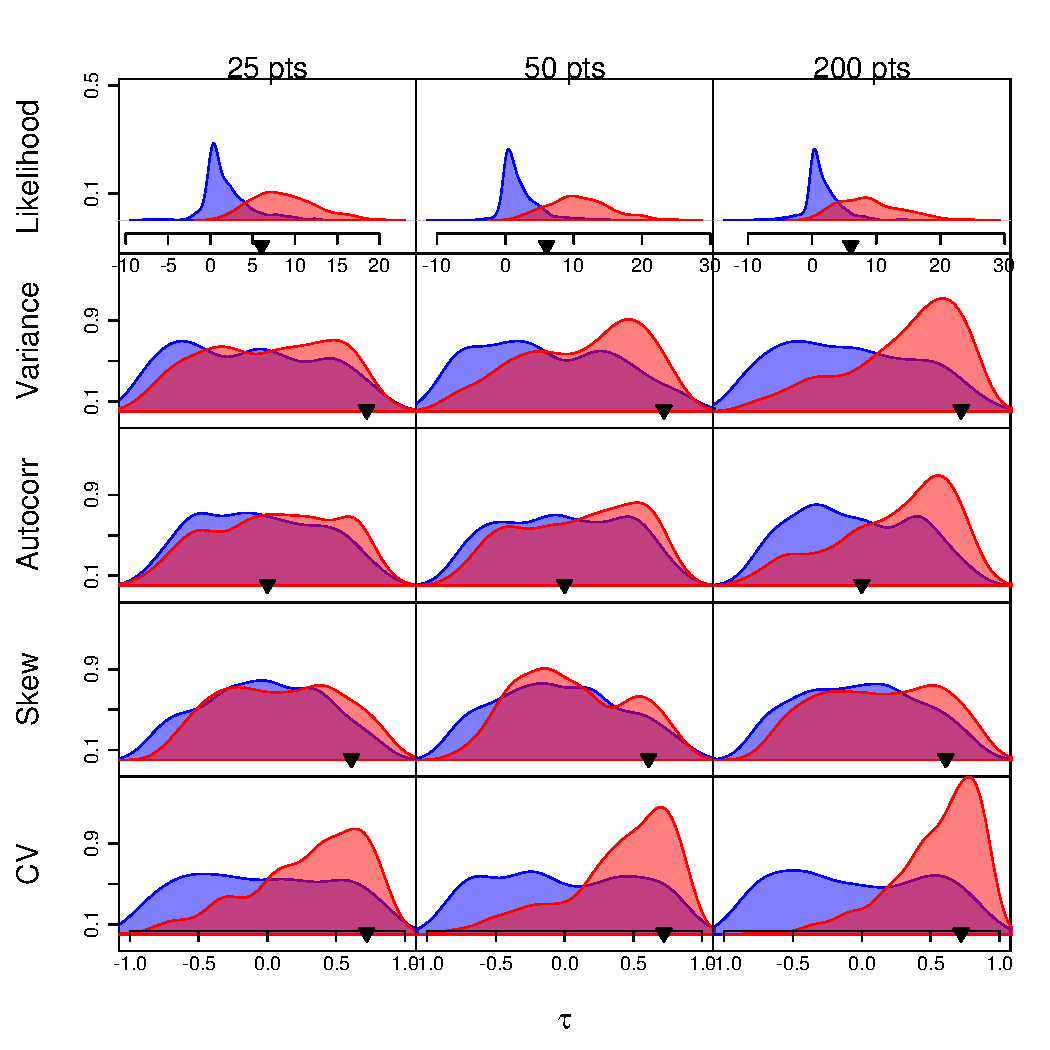
\includegraphics{FigS4.pdf}
  \end{center}
  \caption{Distributions of the indicator statistic as the sampling effort increases in the Glaciation I data.}
  \label{fig:S4}
\end{figure}



The ROC curve indicates the trade off between false alarms and failed detections, 
from which we may choose a threshold value that will allow us to classify the data set as having detected a warning or not.  
For instance, in the case of the \emph{Daphnia} data, the 90\% true-positive, 35\% false-positive rate corresponds with a threshold of 
$\delta = 2.5$.  The observed $\delta=6.0$, clearly above that threshold.  
We can of ask what is the probability of a false alarm or missed event at the observed threshold of 6 as well: \%9.5 false alarm rate.  
While it is possible to classify 


which can guide the classification of a particular system as 
When the curve lies very close to the 1:1 line, there is essentially no information provided by the given warning indicator,
and classifying

To determine whether the data should be considered 


 \section*{ }%bibliography
 \bibliography{/home/cboettig/Documents/bibliographies/library.bib}

 \end{document}



